\section{Combining Unidirectional Consistency Preservation Rules}

\mnote{Make bidirectional transformation synchronizing}
We have introduced that bidirectional transformations, as we assume to be the notion for practically usable transformation specifications, can only be applied after changes to one model and update the other to restore consistency.
This induces a gap to synchronizing transformations, as required in transformation networks, which are able to accept changes made in both models and update both models to restore consistency.
To close this gap, we discuss options to combine the unidirectional consistency preservation rules of a bidirectional transformation, such that it considers changes made to both models and thus acts like a synchronizing transformation.


%%
%% OPTIONS TO COMBINE TRANSFORMATIONS / CPRS
%%
\subsection{Options for Combination}

\mnote{Conflicting concurrent changes}
Some existing work already proposed strategies to synchronize concurrent changes between two models.
For example, some work proposes techniques for processing concurrent changes with \glspl{TGG}~\cite{hermann2012concurrentSynchronization-FASE,orejas2020IncrementalConcurrentSynchronization-FASE}, whereas others define specific algorithms for a general notion of synchronizing transformations according to our given definition~\cite{xiong2013SynchronizingConcurrentUpdates-SoSym,xiong2009parallelUpdates-ICMT}.
All these approaches, however, deal with the more general case that any changes may have been made to the models.
That especially includes conflicting updates by one or more user, which need to be resolved.
Such a resolution may lead to the necessity of reverting one of the changes.

\mnote{Specific concurrent changes in transformation networks}
We are, however, in the situation that transformations do not perform arbitrary changes and that changes of other transformations may need to be revised but not reverted.
For example, it may be necessary to update an attribute value again, because the interval of consistent values of the currently executed transformation is smaller than the one of a transformation executed before.
It will, however, not be necessary to completely revert the modification of the attribute value, because the modification was necessary for another transformation to restore consistency, thus the causal change for which consistency was restored would need to be reverted as well.
Finally, this would result in reverting a user change, which should never happen.

\mnote{Assumed compatibility of relations}
We assume the consistency relations of transformations to be compatible according to \autoref{def:compatibility}, which excludes contradictions that may prevent transformations from being able to find a consistent result for specific changes.
This assumptions reduces the potential conflicts that may occur when changes of different transformations need to be synchronized.

%\mnote{Difference between synchronizing and unidirectional consistency preservation rules}
%A synchronizing consistency preservation rule according to \autoref{def:consistencypreservationrule} receives two models and two changes, one for each of the models, and returns two changes, i.e.:
% \begin{align*}
%     \consistencypreservationrule{\consistencyrelation{CR}{}} : (\metamodelinstanceset{M}{1}, \metamodelinstanceset{M}{2}, \changeuniverse{\metamodel{M}{1}}, \changeuniverse{\metamodel{M}{2}}) \rightarrow (\changeuniverse{\metamodel{M}{1}}, \changeuniverse{\metamodel{M}{2}})
% \end{align*}
%\todo{Maybe add this to correctness formalization: Give example why we need that: both models can be modified due to network, both may need to be modified because if in both models something is added that needs to be reflected in the other, both have to be changed to restore consistency, without reverting one of the changes.}
%We used this rather general notion of a consistency preservation rule between two metamodels to support that both models may have been modified, which is inevitable in a transformation network.
%Additionally, both models may need to be modified to properly consistency.
% It would, however, be a cumbersome task to define the behavior of the transformation, or more precisely its consistency preservation rule, for all potential pairs of changes in both models.
% Furthermore, existing transformation languages usually specify unidirectional consistency preservation rules, thus they only support the propagation of changes made in one model to the other, but not to process changes made to both models at once. Thus, each bidirectional transformation defined in a transformation language actually consists of two consistency preservation rules:
% \begin{align*}
%     \consistencypreservationrule{\consistencyrelation{CR}{},\rightarrow} : (\metamodelinstanceset{M}{1}, \metamodelinstanceset{M}{2}, \changeuniverse{\metamodel{M}{1}}) \rightarrow \changeuniverse{\metamodel{M}{2}}\\
%     \consistencypreservationrule{\consistencyrelation{CR}{},\leftarrow} : (\metamodelinstanceset{M}{1}, \metamodelinstanceset{M}{2}, \changeuniverse{\metamodel{M}{2}}) \rightarrow \changeuniverse{\metamodel{M}{1}}
% \end{align*}

\mnote{Execution of both preservation rules}
A bidirectional transformation according to \autoref{def:bidirectionaltransformation} consists of two unidirectional consistency preservation rules.
We have discussed in \autoref{chap:synchronization:gap:alignment} that it is not possible to extend those consistency preservation rules to be synchronizing such that the execution of a single unidirectional consistency preservation rule restores consistency to all consistency relations after changes to both models.
In fact, it will be necessary to execute both preservation rules at least ones to restore consistency.
There are, however, different options how to apply the rules, each having different benefits and drawbacks.

\mnote{Independent execution and merge}
%In consequence, we usually have two unidirectional consistency preservation rules $\consistencypreservationrule{\consistencyrelation{CR}{},\rightarrow}$ and $\consistencypreservationrule{\consistencyrelation{CR}{},\leftarrow}$ that define how changes are propagated from one model to the other and vice versa, but this is not equivalent to a synchronizing transformation.
We have already sketched two scenarios for executing multiple consistency preservation rules in \autoref{chap:correctness:notions_consistency:preservation}, which can be transferred to the case of executing the two consistency preservation rules of a bidirectional transformation.
A first option is to independently apply the consistency preservation rules and then merge the results.
Imagine models $\model{m}{1}$ and $\model{m}{2}$ and changes to them $\change{\metamodel{M}{1}}$ and $\change{\metamodel{M}{2}}$.
If we apply the two unidirectional consistency preservation rules independently, we get $\change{\metamodel{M}{2}}' = \consistencypreservationrule{\consistencyrelationset{CR}}^{\rightarrow}(\model{m}{1},\model{m}{2}, \change{\metamodel{M}{1}})$ and $\change{\metamodel{M}{1}}' = \consistencypreservationrule{\consistencyrelationset{CR}{}}^{\leftarrow}(\model{m}{2}, \model{m}{1}, \change{\metamodel{M}{2}})$.
It is, however, not guaranteed that $\tupled{\change{\metamodel{M}{1}}'(\change{\metamodel{M}{1}}(\model{m}{1})), \change{\metamodel{M}{2}}'(\change{\metamodel{M}{2}}(\model{m}{2}))}$ is consistent to $\consistencyrelationset{CR}$.
It is even not guaranteed that the changes, such as $\change{\metamodel{M}{1}}$ and $\change{\metamodel{M}{1}}'$ can be concatenated at all, since $\change{\metamodel{M}{1}}'$ was generated for $\model{m}{1}$ rather than $\change{\metamodel{M}{1}}(\model{m}{1})$.
An example may be that $\change{\metamodel{M}{1}}$ removes an element from $\model{m}{1}$, which $\change{\metamodel{M}{1}}'$ changes.
Even if the change is still defined for that changed model, the result may not be consistent because the necessary change produced by $\consistencypreservationrule{\consistencyrelationset{CR}}^{\rightarrow}$ cannot be applied anymore.
%For example, $\change{\metamodel{M}{1}}'$ may add an element that $\change{\metamodel{M}{1}}$ already added.
%Then the resulting model may be invalid or, if the element is only added once, this may result in the missing existence of unique corresponding elements to build a witness structure for consistency.
Thus simply merging the individually produced changes does not necessarily lead to a consistent result.

\mnote{Sequential execution}
Another option is to sequence the execution, thus first generating $\change{\metamodel{M}{2}}' = \consistencypreservationrule{\consistencyrelationset{CR}}^{\rightarrow}(\model{m}{1},\model{m}{2}, \change{\metamodel{M}{1}})$ as before.
$\tupled{\change{\metamodel{M}{1}}(\model{m}{1}), \change{\metamodel{M}{2}}'(\model{m}{2})}$ is consistent due to correctness of $\consistencypreservationrule{\consistencyrelationset{CR}}^{\rightarrow}$.
Afterwards, we apply the second consistency preservation rule to the the new consistent models and the original change to $\model{m}{2}$, thus $\change{\metamodel{M}{1}}' = \consistencypreservationrule{\consistencyrelationset{CR}}^{\leftarrow}(\change{\metamodel{M}{2}}'(\model{m}{2}), \change{\metamodel{M}{1}}(\model{m}{1}), \change{\metamodel{M}{2}})$.
As a result, we receive $\tupled{\change{\metamodel{M}{1}}'(\change{\metamodel{M}{1}}(\model{m}{1})), \change{\metamodel{M}{2}}(\change{\metamodel{M}{2}}'(\model{m}{2}))}$, which is consistent to $\consistencyrelationset{CR}$.
This means that $\change{\metamodel{M}{2}}$ is not applied to $\model{m}{2}$ anymore, to which the changes were made originally, but needs to be applied to $\change{\metamodel{M}{2}}'(\model{m}{2})$.
It is again unclear whether the change can still be applied to that state, i.e., whether $\change{\metamodel{M}{2}}$ is defined for $\change{\metamodel{M}{2}}'(\model{m}{2})$, like in the merge example above.
If, however, the changes are applicable, then we have the guarantee that all original changes are reflected, as they were applied to the models, and that the resulting models are consistent, because of the correctness of the consistency preservation rules.
%An example may be that $\change{\metamodel{M}{2}}'$ removes an element from $\model{m}{2}$, which $\change{\metamodel{M}{2}}$ changes.
%\todo{Revise change definition to be partial}

\mnote{Sequential execution with less drawbacks}
Both discussed options have the drawback that they cannot guarantee to produce a result, as it is possible that the involved changes cannot be concatenated.
In addition, the first option of independently applying the consistency preservation rules and then merging the results cannot even give a guarantee that if changes can be concatenated the resulting models are consistent.
Thus, we do not pursue that approach anymore.
In the following, we further discuss the second option of sequencing the execution of the consistency preservation rules.

% \mnote{Goal is to preserve all original changes}
% We, however, want to ensure that both original changes are applied to the models and consistency preservation rules can react to them.
% Thus, we aim to find an approach that allows the unidirectional consistency preservation rules to also deal with the situation that the both models have been modified to emulate a synchronizing rule.


%%%
%%% SEQUENCING OF CPRS
%%%
\subsection{Sequencing of Consistency Preservation Rules}
\label{chap:synchronization:combination:sequencing}

\begin{figure}
    \centering
    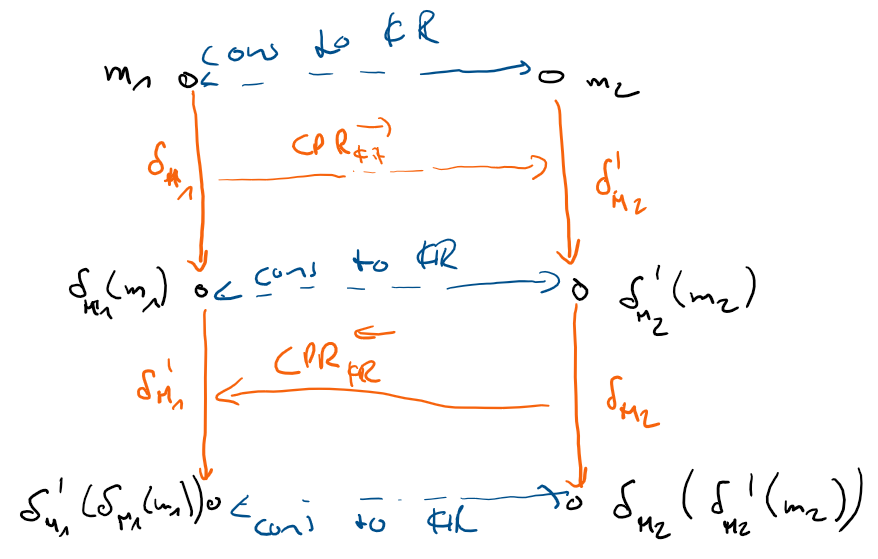
\includegraphics[width=0.8\textwidth]{figures/correctness/synchronization/sequencing_schema.png}
    \caption[Sequencing unidirectional consistency preservation rules]{Schema for sequencing unidirectional consistency preservation rules after concurrent changes.}
    \label{fig:synchronization:sequencing_schema}
\end{figure}

\mnote{Changes affecting disjoint element sets}
The sequential application of original changes and execution of consistency preservation rules as explained in the previous section is depicted schematically in \autoref{fig:synchronization:sequencing_schema}.
It has two important properties. 
First, it ensures that all original changes are applied to the models and, second, it guarantees that the resulting models are consistent.
It is, however, only applicable in specific situations.
The optimal case, in which the approach is always applicable, is if $\consistencypreservationrule{\consistencyrelationset{CR}}^{\rightarrow}$ produces changes for the second model that affect a disjoint set of elements in $\consistencyrelationset{CR}$ compared to the original changes to the second model $\change{\metamodel{M}{2}}$.
If two changes affect completely disjoint sets of elements, they can obviously be consecutively applied.
It would even not make a difference in which order they are applied then.

\begin{figure}
    \centering
    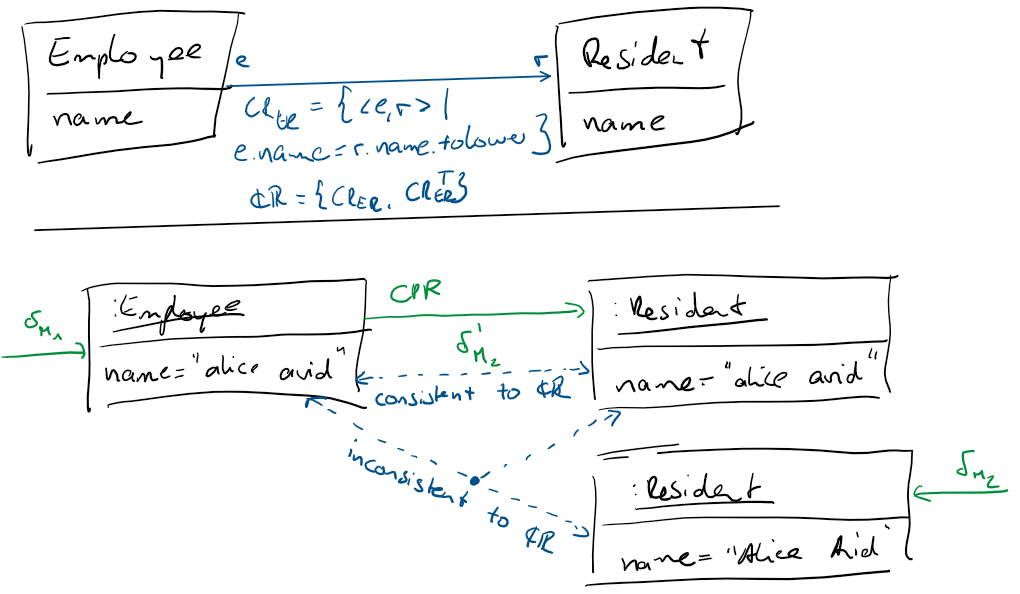
\includegraphics[width=\textwidth]{figures/correctness/synchronization/non_transformability.png}
    \caption[Non-transformability in sequencing scenario]{Example for non-transformability when sequencing the application of unidirectional consistency preservation rules and concurrent changes.}
    \label{fig:synchronization:non_transformability}
\end{figure}

\mnote{Issues when sequencing preservation rule application}
Unfortunately, the changes $\change{\metamodel{M}{2}}'$ produced by $\consistencypreservationrule{\consistencyrelationset{CR}}^{\rightarrow}$ and the original ones produced by other transformations $\change{\metamodel{M}{2}}$ do not necessarily affect disjoint sets of elements.
In that case, two problems can occur:
\begin{properdescription}
    \item[Non-Applicability:] The most obvious problem, which we have already discussed, is that the original change to the second model $\change{\metamodel{M}{2}}$ cannot be applied to the model changed by $\change{\metamodel{M}{2}}'$ as the result of $\consistencypreservationrule{\consistencyrelationset{CR}}^{\rightarrow}$. 
    This can, for example, happen when $\change{\metamodel{M}{2}}'$ removes an element that is affected by $\change{\metamodel{M}{2}}$.
    Due to the change of the element in $\change{\metamodel{M}{2}}$, it is part of a condition element in another transformation that was executed before.
    Since $\consistencypreservationrule{\consistencyrelationset{CR}}^{\rightarrow}$ removed that element, the condition element exists no longer anyway, thus this removal has to be propagated back by the transformation that originally introduced the change in $\change{\metamodel{M}{2}}$.
    In consequence, the modification in $\change{\metamodel{M}{2}}$ can simply be ignored.
    In the worst case, all elements affected by $\change{\metamodel{M}{2}}$ were removed by $\change{\metamodel{M}{2}}'$, then, in fact, all changes in $\change{\metamodel{M}{2}}$ can be ignored, because all condition elements of the involved consistency relations were removed.
    Thus, we can always ensure that the changes, at least those that are still relevant, can still be applied.
    
    \item[Non-Transformability:] Even if the changes $\change{\metamodel{M}{2}}$ can be applied to $\change{\metamodel{M}{2}}'(\model{m}{2})$, this does still not guarantee that $\consistencypreservationrule{\consistencyrelationset{CR}}^{\leftarrow}$ is able to process the given changes.
    In fact, this requirement applies to all changes, thus even original user changes, but there are special circumstances in this situation that make it prone to not being able to transform the changes.
    Whenever $\change{\metamodel{M}{2}}'$ adds condition elements that were already added by $\change{\metamodel{M}{2}}$, their concatenation can lead to a duplication of those elements.
    Consider the scenario depicted in \autoref{fig:synchronization:non_transformability} with consistency relations $\consistencyrelationset{CR} = \setted{\consistencyrelation{CR}{ER}, \consistencyrelation{CR}{ER}^T}$. 
    An employee \enquote{alice avid} is added by the original change to $\model{m}{1}$.
    The consistency preservation rule then generates an appropriate resident with the same name to fulfill the consistency relation.
    Applying the original change to $\model{m}{2}$ then leads to the addition of resident \enquote{Alice Avid}, which was generated by another transformation, e.g., the one that created an appropriate person and changed the capitalization of the name.
    Now it is impossible for $\consistencypreservationrule{\consistencyrelationset{CR}}^{\leftarrow}$ to generate a change $\change{\metamodel{M}{1}}'$ for the first model to restore consistency. The employee corresponds to both residents, as both fulfill the constraint of the consistency relation. 
    But there is no additional employee that could be added to achieve a unique mapping between corresponding elements.
    A synchronizing transformation would have been able to produce a consistent result by simply performing no additional changes, as the originally added resident is already consistent to the originally added employee.
    In consequence, if the unidirectional consistency preservation rule had known that the resident was already added, it would not have performed any changes.
\end{properdescription}

\mnote{Non-transformable changes of users unavoidable}
As remarked before, the situation that certain changes cannot be processed by the consistency preservation rules cannot be avoided. 
If the user had added the second resident in the previous scenario, there would have also been no possibility for the consistency preservation rule to generate changes that restore consistency.
The difference is, however, that in this case it is fine that consistency preservation cannot find a result, whereas in case of the scenario discussed above, the original changes could have been reasonably processed to a consistent result, if the unidirectional consistency preservation rule would have considered that there already was a change that restored consistency.

\mnote{Necessity to process inconsistent inputs}
In consequence, it is inevitable that consistency preservation rules need to be able to deal with the situation that the second model was already modified, such that the given models are not initially consistent, to reflect the changes that already have been made and integrate them into consistency preservation.
This means that we finally have to relax our requirements for the input of consistency preservation rules to be able to consider the changes to both models.
This means that we need to make further requirements to the preservation rules, because we do not assume the consistency preservation rules to produce results for inputs that are not consistent.
We have already given examples where it is not possible to restore consistency by one unidirectional consistency preservation rule after changes in both models.

\mnote{Relaxed notion affecting number of executions}
Before we define a precise notion of further requirements to consistency preservation rules that accept inconsistent inputs, we first discuss how often it may be necessary to execute both consistency preservation rules to restore consistency, as this directly affects the requirements we have to define.

%Optimalfall: d2' und d2 erzeugen Änderungen für Elemente, die disjunkte Mengen von Condition Elements betreffen. Dann können sie beliebig sequentialisiert werden und erzeugen konsistente Ergebnisse.

% Problemfälle:
% d2' erzeugt Änderungen, die sich nicht auf d2 anwenden lassen
% d2' erzeugt Änderungen, die sich auf Condition Elemente beziehen, die von d2 geändert werden
% d2' und d2 erzeugen Änderungen, die zusammen neue Condition Elements induzieren

% \begin{itemize}
%     \item In the best case we would apply changes to model 1, then execute the first preservation rule to change model 2 (so they are consistent then again) and then apply the changes to model 2 and execute the second preservation rule, such that they are then consistent again.
%     \item What comes in mind directly: For sure, this could result in the situation that changes are reverted, because the change to 1 propagated by 1 -> 2 changes a value which is changed by back by change to 2 and then reverted back by 2 -> 1. But even a synchronizing transformation would have to select either of the values in that case and revert one the changes, so there is already an underlying problem of the relations that may not be compatible
%     \item It is however unclear whether the changes to model 2 can still be applied after applying the changes of the transformation 
%     \item We therefore make a case distinction over all possible combinations of changes to be executed one after another.
%     \item Especially, we want to find out where there are conflicts if changes to model 2 are applied before 1 -> 2 changes. This allows us to encode 1 -> 2 in a way that it is able to deal with it instead of having the problem of not being able to apply changes to model 2
% \end{itemize}

% Kann d2 auf d2' angewendet werden? Was sind mögliche Probleme?
% %Wir können Sequentialisieren, aber dann sind Änderungen potentiell nicht mehr propagierbar (und wenn die CPR es doch tun, weil sie für die Eingabe undefiniert sind und irgendwas tun, kommt Quatsch raus).

% 1. Nicht Anwendbarkeit: Element, auf das Änderung angewendet werden soll, existiert nicht mehr. D.h. das Element wurde durch die CPR entfernt, was nötig war, um die entsprechende Konsistenzrelation zu erfüllen. Die Änderung die über einen anderen Pfad kam, kann nicht mehr angewendet werden. Das Condition Element ist nicht mehr vorhanden, also muss diese Löschung zurückpropagiert werden, damit auch entsprechend der anderen Konsistenzrelationen die korrespondierenden Condition Elements entfernt werden -> Änderung wird ignoriert und die Löschung wird propagiert
% 2. Nicht Propagierbarkeit (gilt generell für die Propagierbarkeit von Änderungen, nicht nur in diesem Szenario, auch bei Nutzeränderungen): Wenn alle Änderungen angewendet sind, kann der Zielzustand so sein, dass d1(m1) nicht so angepasst werden, dass Konsistenz wiederherstellt wird. Dies ist insbesondere dann der Fall, wenn für d2(d2'(m2)) kein Modell in IM1 existiert, sodass es eine valide Witness-Struktur gibt. Das ist dann der Fall, wenn nicht für jedes Condition Element ein eindeutiges korrespondierendes gefunden werden kann, also entweder aufgrund der Elemente in d2(d2'(m2)) in einem m1 Elemente vorkommen müssen, die durch eine Konsistenzregel ein weiteres Condition Element in d2(d2'(m2)) benötigen würden, oder es kein m1 gibt, sodass eine eindeutige Zuordnung möglich ist, also in d2(d2'(m2)) quasi doppelte Elemente vorkommen

% Ersteres wäre bspw. der Fall, wenn ein zweiter Resident eingefügt wird, dafür entsprechend ein zweiter Employee erzeugt werden muss, aber bei zwei Employees (warum auch immer) immer ein dritter Resident erzeugt werden muss, durch eine weitere Konsistenzrelation. Dies wäre jedoch auch ein Problem, wenn der Nutzer eine solche Änderung macht, da dann die CPR gar nicht in der Lage ist unidirektional Konsistenz herzustellen. Daher können wir mit solch einer Art von  Konsistenzrelationen sowieso per se nicht umgehen. Wie bereits gesagt, kann man das in der Praxis dennoch erlauben und verliert dann gewisse Garantien bzgl. Konsistenz oder Terminierung. Der Entwickler muss das halt einfach richtig umsetzen.
% Dieses Problem ließe sich noch durch mehrfache Ausführung der Transformationen lösen, da es immer noch Modelle gibt, die diese Änderung reflektieren und konsistent sind, muss eben nur die Transformationen dafür lange genung ausführen.

% Zweiteres wäre beispielsweise ein doppelter Resident, für den kein konsistentes Employee-Modell erzeugt werden kann.
% Das Vorkommen doppelter Elemente lässt sich auch nicht durch mehrfache Ausführung der CPR auflösen (außer man löscht eines der Elemente wieder).
% Hier ist das zugrunde liegende Problem, dass mehrfach ein Element erzeugt wurde, was eigentlich das gleiche sein soll.
% Eine synchronisierende Transformation könnte an dieser Stelle berücksichtigen, dass d2 bereits entsprechende Elemente einfügt, sodass in d2' nicht zusätzliche Erzeugungen generiert werden müssen, um eine valide Witness-Struktur zu induzieren.
% Die unidirektionale CPR sieht diese Änderung jedoch nicht und somit passiert die Hinzufügung doppelt.
% Um das zu Vermeiden müsste die CPR berücksichtigen, dass d2 bereits entsprechende Änderungen macht.

% Go on here \dots


% Wenn wir die unidirektionalen CPR sequentialisieren (also erst d2' erzeugen, dann d2 darauf anwenden), kann es sein, dass d2'(m2) Änderungen an Condition Elements in m2 vornimmt oder neue hinzufügt, um Konsistenz wiederherzustellen, die ebenfalls von d2 eingefügt werden, sodass es nicht mehr möglich ist, durch die rückwärtige CPR Änderungen vorzunehmen, die eine valide Witness-Struktur induzieren.
% Z.B. könnte d2'(m2) einen Resident hinzufügen, der bereits durch d2 eingefügt wurde (weil er über einen anderne Pfad erstellt wurde, siehe \autoref{fig:synchronization:duplicate_creation_example}). Wird nun d2 auf d2'(m2) angewendet, würde ggf. in einem Container, in dem die Residents gespeichert werden, zwei Residents mit gleichem Namen eingefügt. Für diese kann aber keine Änderung in m1 (sei es das Employee-Modell) erzeugt werden, durch die eine valide Witness-Struktur entsteht. Das Einfügen eines zweiten Employee mit dem gleichen Namen führt dazu, dass jeder Employee und jeder Resident zu zwei Residents bzw. Employees korrespondiert, was keine eindeutige Witness-Struktur induziert.
% Um dies zu vermeiden, müssen die CPR sicherstellen, dass in den Änderungen am anderen Modell nicht bereits entsprechende Condition Elements erzeugt wurden.
% Alle anderen Änderungen sind unproblematisch, da Änderungen die d2 an bestehenden Condition Elements, die nicht zu neuen Condition Elements führen, durchführt mittels 2->1 propagiert werden können, indem die Condition Elements in m1 angepasst werden.

% Insgesamt ist die Situation die gleiche, als würde ein Nutzer eine entsprechende Änderung machen. Auch er kann natürlich einen zweiten Resident mit demselben Namen einführen. Hier würde die CPR selbstverständlich fehlschlagen. Während das für Nutzeränderungen erwüscht ist, da die doppelte Erzeugung desselben Elementes hier schon vom Nutzer durchgeführt wurde und für einen entsprechende Nutzeränderung kein konsistentes Modell generiert werden kann, ist dies innerhalb des Transformationsnetwerkes unerwünscht, da die CPR natürlich eine konsistente Modellmenge finden können und die doppelte Erzeugung lediglich daher kommt, dass die Transformationen nicht, wie verlangt, synchronisieren sind. In letztem Fall wäre sichergestellt, dass nach entsprechenden Änderungen an beiden Modellen (also Erzegung von Employee in einem, Erzeugung des passenden Resident im anderen) keine Änderungen gemacht werden, da bereits eine passende Witness-Struktur vorhanden ist.
% Die unidirektionalen CPR schaffen das jedoch nicht, da Ihnen die entsprechende Information fehlt.

% \paragraph{Concatenation of Changes}
% WAS PASSIERT EIGENTLICH BEI CHANGE CONCATENATION?
% Bis jetzt haben wir Änderungen immer nur auf den Zustand eines Modells angewandt, für den sie auch generiert waren. Ein Change kann jedoch von seiner Definition her auch auf andere Zustände angewandt werden. Die Frage ist, wie er sich dabei verhält. Die Definition macht dazu erstmal keine Aussage, d.h. er könnte im Prinzip beliebigen Quatsch machen. Natürlicherweise würde man aber erwarten, dass er dieselben Änderungen an Modellen durchführt (Einfügen/Löschen von Objekten, Ändern von Attributen/Referenzen usw.), soweit dies möglich ist. Zumindest wenn die jeweiligen Elemente vorhanden sind, auf die sich die Änderungen beziehen, sollte die Änderung das gleiche ausführen.
% Da wir das nicht präzise formulieren können, kommen wir nicht umhin, dass d2' auf Basis von d2(m2) erzeugt wird. Also spricht auch das gegen Sequentialisierung.


%%%
%%% NON-TERMINATION
%%%
\subsection{Execution Bounds} % for Bidirectional Transformations}
\label{chap:synchronization:combination:bounds}

\begin{figure}
    \centering
    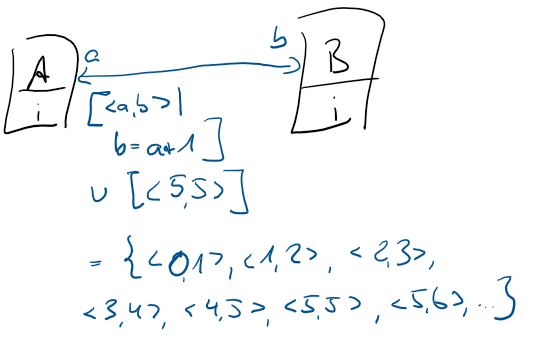
\includegraphics[width=0.7\textwidth]{figures/correctness/synchronization/multiple_unidirectional_execution.png}
    \caption[Multiple execution of consistency preservation rules]{A consistency relation requiring multiple executions of unidirectional consistency preservation rules to find a consistent result.}
    \label{fig:synchronization:multiple_unidirectional_execution}
\end{figure}

\mnote{Unidirectional preservation rules cannot always be correct}
Correctness of unidirectional consistency preservation rules ensures that after executing such a rule the resulting models are consistent.
It is easy to see that this correctness notion cannot be fulfilled for certain sets of consistency relation sets.
This is exemplified at the artificial scenario depicted in \autoref{fig:synchronization:multiple_unidirectional_execution}.
We consider two consistency relations $\consistencyrelation{CR}{1}$ and $\consistencyrelation{CR}{2}$ and their transposed relations, i.e., $\consistencyrelationset{CR} = \setted{\consistencyrelation{CR}{1}, \consistencyrelation{CR}{1}^T, \consistencyrelation{CR}{2}, \consistencyrelation{CR}{2}^T}$.
$\consistencyrelation{CR}{1}$ requires that for each \modelelement{A} an instance of \modelelement{B} exists, which has the same value of $i$ incremented by $1$.
The only exception is that if $i$ in \modelelement{A} is $4$ (or any other arbitrary value), then no corresponding element \modelelement{B} is required.
$\consistencyrelation{CR}{2}$ requires that for each \modelelement{A} an instance of \modelelement{B} exists, which has the same value of $i$.
We want to define a bidirectional transformation of two unidirectional consistency preservation rules $\consistencypreservationrule{\consistencyrelationset{CR}}^{\rightarrow}$ for propagating changes in models with instances of \modelelement{A} to one with instances of \modelelement{B} and $\consistencypreservationrule{\consistencyrelationset{CR}}^{\leftarrow}$ to propagate changes in the opposite direction. 

\mnote{Example scenario}
Consider the following scenario: If an \modelelement{A} with $i = 0$ is added to an empty model, $\consistencypreservationrule{\consistencyrelationset{CR}}^{\rightarrow}$ cannot perform any changes in an (also empty) model with instances of \modelelement{B} that restore consistency.
Because of $\consistencyrelation{CR}{1}$, a \modelelement{B} with $i = 1$ has to be created, and because of $\consistencyrelation{CR}{2}$, a \modelelement{B} with $i = 0$ has to be created.
While this also fulfills $\consistencyrelation{CR}{1}^T$, the existence of \modelelement{B} with $i = 1$ requires the existence of an \modelelement{A} with $i = 1$ due to $\consistencyrelation{CR}{2}^T$.
Since $\consistencypreservationrule{\consistencyrelationset{CR}}^{\rightarrow}$ cannot modify the model with instances of \modelelement{A}, it is impossible for $\consistencypreservationrule{\consistencyrelationset{CR}}^{\rightarrow}$ to restore consistency in that case.

\mnote{Multiple executions leading to consistent result}
Allowing the consistency preservation rules to react to each other multiple times can, however, lead to a consistent result.
If $\consistencypreservationrule{\consistencyrelationset{CR}}^{\leftarrow}$ adds an \modelelement{A} with $i = 1$ in response to the previous execution of $\consistencypreservationrule{\consistencyrelationset{CR}}^{\rightarrow}$, all consistency relations except $\consistencyrelation{CR}{1}$ are fulfilled.
$\consistencypreservationrule{\consistencyrelationset{CR}}^{\rightarrow}$ can then create a \modelelement{B} with $i = 2$, which is iteratively processed by $\consistencypreservationrule{\consistencyrelationset{CR}}^{\leftarrow}$.
This process terminates as soon as $\consistencypreservationrule{\consistencyrelationset{CR}}^{\rightarrow}$ adds a \modelelement{B} with $i = 5$, as then $\consistencyrelation{CR}{1}^T$ is also fulfilled, because it does not require a corresponding \modelelement{A} for a \modelelement{B} with $i = 5$.

\mnote{Arbitrary high number of necessary executions}
We have seen that it is possible to execute unidirectional consistency preservation rules multiple times to achieve a consistent state and that it is not always possible to ensure consistency with only one execution of such a rule.
In fact, the number of necessary execution of consistency preservation rules can be arbitrarily high.
The value of $5$ in $\consistencyrelation{CR}{1}$ of the example can be exchanged by an arbitrary high value requiring an arbitrary high number of executions.
This may only be circumvented if we required that $\consistencypreservationrule{\consistencyrelationset{CR}}^{\rightarrow}$ must perform changes such that $\consistencypreservationrule{\consistencyrelationset{CR}}^{\leftarrow}$ can then restore consistency with a single execution.
In our scenario this would mean that $\consistencypreservationrule{\consistencyrelationset{CR}}^{\rightarrow}$ adds all \modelelement{B} with $i \leq 5$.
Anyway, such a behavior requires a relaxation of the correctness requirement for consistency preservation rules, because $\consistencypreservationrule{\consistencyrelationset{CR}}^{\rightarrow}$ can never result in a consistent state.

\mnote{Preservation rules complete partial condition elements}
Additionally, it may be desired that elements of a consistency relation are created by a consistency preservation rule, although a condition element was only created partially so far.
In that case, both the partial condition element has to be completed in one model and the corresponding condition element in the other model have to be created.
Thus changes in both models are required, which can only be achieved by executing both consistency preservation rules and accepting that the first executed one does not return consistent models.
An example for such a scenario could be the consistency relation between components in \gls{PCM} and their realization as a package and component in Java.
It may be desired that as soon as a package at a specific place, e.g., a \enquote{components} package, or with a specific name, e.g., containing \enquote{Component}, is created in the Java code, this is identified as a component, thus creating the component in the \gls{PCM} model as well as the implementation class in Java.
In that case, there is no complete condition element created in Java, because this would also require the existence of an appropriate class.
If the elements shall still be created, both models have to be changed, thus the first consistency preservation rule introduces the \gls{PCM} component which introduces an inconsistency between the models, as the corresponding Java class is missing, which is then corrected by the second consistency preservation rule.

\mnote{Necessity of termination guarantee}
Finally, it is questionable whether such scenarios should be considered in the formal framework or if it should be up to a developer to implement such a scenario without having specific guarantees regarding termination of the consistency preservation rules or regarding consistency of the models after executing the rules a specific number of times.
Since we need to relax the requirement of consistency preservation rules to always produce consistent results after one execution in the synchronization scenario where both models have been modified, we will allow the consistency preservation rules to be executed more than once anyway.
Regarding the example in \autoref{fig:synchronization:multiple_unidirectional_execution}, if we started with an \modelelement{A} with $i = 6$ and let the consistency preservation rules operate as discussed above, always adding the elements with $i$ incremented by one, this process would never terminate.
We thus need to ensure that such an execution terminates.
Since the consistency preservation rules depend on each other, this will, however, be a property of the bidirectional transformation rather than the individual consistency preservation rule.

% Wie bei Orchestrierung gesehen, kann es im Allgemeinen notwendig sein CPRs mehrfach auszuführen, da die aufeinander reagieren müssen, um eine konsistente Modellmenge "auszuhandeln".
% Dasselbe kann bei zwei unidirektionalen Transformationen passieren. Während eine synchronisierende Transformation beliebige Änderungen an beiden Modellen machen kann, kann es sein, dass unidirektionale Transformationen mehrfach aufeinander reagieren müssen, um das gleiche zu erreichen.


% Siehe \autoref{fig:synchronization:multiple_unidirectional_execution}: Es gibt zwei Relationen (und deren transponierte). Die eine Relation ist erfüllt, wenn für jedes A mit einer Zahl ein B mit der Zahl um eins höher vorkommt, außer A ist 5 (oder eine bel. andere Zahl), dann darf B auch 5 sein (und umgekehrt). Die andere Relation ist erfüllt, wenn für jedes A ein B mit der gleichen Zahl existiert (und umgekehrt).
% Wird nun A(i=0) in das Modell eingefügt, wird zur Erfüllung der Relationen B(i=1) und B(i=0) von der CPRr eingefügt.
% Daraufhin fügt die CPRl A(i=1) ein, da sonst $CR_2$ nicht erfüllt ist.
% Nun fügt CPRr wiederum B(i=2) ein, damit $CR_1$ erfüllt ist usw.
% Dies geht bis CPRl A(i=5) einfügt, denn nun ist auch $CR_1$ erfüllt.
% Es braucht mehrere Durchläufe um dieses Ergebnis zu erhalten.

% Das folgende ist alles intuitiv gesprochen, funktioniert so nicht.
% ERKENNTNIS: Wir können von einer unidirektionalen CPR i.A. gar nicht verlangen, dass sie Konsistenz bzgl. aller Relationen herstellt.
% Ziel ist nur, dass sie die Konsistenzrelationen in Vorwärtsrichtung wiederherstellt, in Rückwärtsrichtung nicht vollständig.
% Bspw. für ein Insert fügt sie Elemente hinzu, bei Änderung passt sie Elemente an. Bei einer Löschung ist die rückwärtige Konsistenzrelation nicht erfüllt, hier muss aber die CPR vorwärts löschen, d.h. wir verlangen, dass Elemente die vorher schon im Zielmodell waren und immer noch sind, auch konsistent sind bzgl. aller Relationen bzgl. der sie vorher konsistent waren.
% Auch für eine Änderung gilt das in die Richtung: Wenn ich an m1 was ändere wodurch eine Witness-Struktur in Rückrichtung verletzt wird, muss die vorwärts CPR das wiederherstellen.

% Das bedeutet, die rückwärts CPR muss dann nur noch auf Hinzufügungen oder Änderungen reagieren, die durch die vorwärts CPR gemacht wurden (auch Löschungen?).
% ERKENNTNIS: Wir können noch nicht einmal Terminierung für zwei unidirektionale Transformationen garantieren. Letztendlich haben wir dort wieder das gleiche Problem wie in Netzwerken, wie wir im Orchestrierungs-Kapitel sehen werden. Das Beispiel zeigt, dass es auch keine obere Schranke für die Anzahl aus Ausführungen gibt (je nach Wahl von X sind hier beliebig viele möglich). Wir könnten Sie nur eine gewissen Zeit ausführen lassen und ansonsten konservativ abbrechen.

% ALSO: Entweder lassen wir das zu, dann können wir keine Terminierung erwarten, oder wir fordern halt, dass eine CPR immer in einem Schritt Konsistenz herstellen muss (für alle Relationen) und wenn sie das nicht schafft, wirft sie eben einen Fehler. Dadurch sind manche Fälle ausgeschlossen, aber das macht man üblicherweise ja immer so.

% WAS TUN WIR?
% Wir verlangen das was alle Formalismen bisher verlangen: Eine unidirektionale CPR kann vollständig Konsistenz herstellen. Auch wenn es theoretische Szenarien gibt, in denen das nicht möglich ist, gehen bisher diverse Arbeiten davon aus und in unserer Evaluation (siehe \autoref{chap:correctness_evaluation}) werden wir sehen, dass es auch in unseren Fallstudien der Fall ist.
% AUßERDEM: In der Praxis können wir natürlich solche Szenarien erlauben, auch wenn dann gewisse Eigenschaften auf Basis des Formalismus nicht mehr garantiert sind.
% Wenn der Entwickler die Transformationen so baut, dass deren mehrfache Ausführung immer terminiert, ist das kein Problem. Ein relevantes Beispiel hierfür könnte sein, dass man eine Konsistenzrelation bereits instanziieren möchte, wenn ein Condition Element nur partiell hinzugefügt wurde, d.h., dass in dem Fall Änderungen an beiden Modellen notwendig sind.
% Hierfür könnte der Ablauf wie folgt sein: In Modell 1 wird ein Condition Element partiell instanziiert, CPRr instanziiert dafür ein korrespondierendes Condition Element in Modell 2, woraufhin CPRl das Condition Element in Modell 1 vervollständigt. In diesem Fall ist nach der Ausführung von CPRr keine Konsistenz gegeben, was jedoch gewünscht ist.
% Beispielsweise wird ein PCM Repository auf drei Packages abgebildet. Nun könnte bereits bei der Erzeugung eines Package (mit passendem Namen) das PCM Repository instanziiert werden, woraufhin die zwei weiteren Java Packages erzeugt werden.

% Man könnte hierfür eine passende Monotonie-Eigenschaft definieren, die das Problem jedoch nur unnötig verkompliziert, sodass wir bei der Anforderung bleiben, dass eine CPR Konsistenz zu allen Relationen herstellt.


\subsection{Necessity for Synchronization Extension}

\mnote{Processing inconsistent input models}
In the previous sections, we have discussed that after changes to two models, these changes and the ones produced by consistency preservation rules that restore consistency between these models cannot be sequenced in a way such that we receive consistent models in all cases the consistency preservation rules are able to handle.
We especially found that it is necessary for a unidirectional consistency preservation rule to consider the changes made to the model it is supposed to modify.
Thus, we need to enable consistency preservation rules to deal with the situation that the input models are inconsistent.
In our current definition, no behavior of a consistency preservation rule and the encapsulating bidirectional transformation for such a situation is defined.
Thus, we discuss an appropriate extension of bidirectional transformations that support this scenario of synchronization in the following section.

\mnote{Guaranteeing termination}
Additionally, we found that it can be required that consistency preservation rules need to be executed multiple times.
This is obviously necessary to make bidirectional transformation synchronizing, thus we will especially consider how to achieve execution bounds, such that termination of multiple executions of the consistency preservation rules of a bidirectional transformation is guaranteed.


% Necessity for extension of BX to make them synchronizing
% Derive that we need transformations that are able to deal with inconsistent input models

% Wir müssen annehmen, dass m2 nicht konsistent ist und dann Fallunterscheidung machen. Aber welche abgeschwächte Garantie können wir fordern, sodass die Ausführung in beide Richtungen immer noch zu Konsistenz führt?
% Das beantworten wir in der folgenden Section.




%%%%
%%%% VERSCHIEDENE VERSUCHE FÜR STRATEGIEN ZUR KOMBINATION VON CPRS
%%%%

% \subsection{Consideration at Condition Element Level}
% % CONSIDERATIONS DO NOT WORK PROPERLY
% \begin{itemize}
%     \item Unidirectional synchronizing: correct if applied to changes d1 to m1, but produces changes d2' that can be applied to d2(m2) as well, and vice versa produces changes d1' for changes d2 to model m2 that can be applied to d1(m1) as well. (Property: Sequentializability, produced changes can handle arbitrary other changes added before)
%     \item For each condition element in d1(m1), i.e., each element for which a consistency relation applies, and for each condition element in d2'(m2), we find exactly one corresponding element in the other model (this is what correctness means). Additionally, in d2'(d2(m2)) $\cap$ d2'(m2), i.e. those elements that are not affected by d2, we also find corresponding 
    
%     \item Take all condition elements in m1 and m2. Take all those for which still only one corresponding condition element exists between m1 and d2(m2), i.e. all the ones not affected by d2. For all of them present in d1(m1) and d2'(d2(m2)), there is still exactly one corresponding condition element. For the ones in d1(m1), which were not in m1, there is a corresponding element in d2'(d2(m2)) and for the ones in d2'(m2), which are also present in d2'(d2(m2)), there is one in d1(m1).
%     \item What if d2'(d2(m2)) produces a new condition element that was not present in m2 and d2(m2) and d2'(m2)? We need to show that this cannot occur?
%     \item Non-synchronizing: d1 and d2 may induce violations of consistency relations. d1' and d2' restore fulfillment of these consistency relations. We consider how consistency relations can be violated when we put d2 in front of d2' and d1 in front of d1' other than in the case when its applied directly.
% \end{itemize}


% \subsection{Versuch über ursächliche Condition Element Änderungen zu unterscheiden}
% Fälle:
% 1. Condition Element wird neu erzeugt
% 2. Condition Element wird geändert, sodass nun ein anderes Element der gleichen Condition vorhanden ist
% 3. Condition Element wird gelöscht
% Es können bei einem Change mehrere davon bzgl. verschiedener Conditions auftreten (also bzgl. verschiedene Consistency Relations)

% Fall 1: Die Vereinigung der Condition Elements aus d2(m2) und d2'(m2) ist gleich derer in d2'(d2(m2)). Somit wird durch die Kombination kein neues Condition Element eingeführt, für das Konsistenz hergestellt werden müsste.

% Fall 2: Die Vereinigung der Condition Elements aus d2(m2) und d2'(m2) ist ungleich derer in d2'(d2(m2)). Somit wird durch die Kombination ein neues Condition Element eingeführt, für das Konsistenz hergestellt werden müsste.

% NEUE STORY:

% Allgemeine Betrachtung von Änderungen: Es geht immer darum, dass Condition Elemente geändert/gelöscht/hinzugefügt wurden und die CPR entsprechend reagieren muss, um das Vorhandensein einer entsprechenden Witness-Struktur zu garantieren. Dabei können entsprechend folgende Fälle auftreten:
% 1. Änderungen führen dazu, dass ein neues Condition Element im Modell existiert, dass zuvor nicht vorhanden war.
% 2. Änderungen führen dazu, dass Elemente eines bereits vorhandenes Condition Elementes geändert werden und dadurch ein andere Condition Element derselben Condition instanziieren.
% 3. Änderungen führen dazu, dass ein vorher existierendes Condition Element nicht mehr im Modell auftaucht.

% Es gibt hierzu drei entsprechende Reaktionen der CPR:
% 1. Im anderen Modell werden, falls nicht vorhanden, entsprechende Elemente erzeugt, um für das neue Condition Element ein eindeutiges korrespondierendes Condition Element zu erzeugen und somit eine Witness-Struktur aufzubauen. (Erzeugungs-Propagation)
% 2. Das gem. Witness-Struktur korrespondierende Condition Element im anderen Modell wird so angepasst, dass wieder eine valide Witness-Struktur entsteht. (Änderungs-Propagation)
% 3. In dem anderen Modell werden die Elemente des korrespondierenden Condition Elementes entfernt (oder zumindest Teile davon), sodass entsprechend der Konsistenzregeln keine weiteren Elemente vorhanden sein müssen, d.h. wieder eine valide Witness-Struktur vorhanden ist.

% % DIE FOLGENDEN ZWEI PARAGRAPHEN SIND NUN BEI DER STRIKTEN SEQUENTIALISIERUNG
% Wenn wir die unidirektionalen CPR sequentialisieren (also erst d2' erzeugen, dann d2 darauf anwenden), kann es sein, dass d2'(m2) Änderungen an Condition Elements in m2 vornimmt oder neue hinzufügt, um Konsistenz wiederherzustellen, die ebenfalls von d2 eingefügt werden, sodass es nicht mehr möglich ist, durch die rückwärtige CPR Änderungen vorzunehmen, die eine valide Witness-Struktur induzieren.
% Z.B. könnte d2'(m2) einen Resident hinzufügen, der bereits durch d2 eingefügt wurde (weil er über einen andere Pfad erstellt wurde, siehe \autoref{fig:synchronization:duplicate_creation_example}). Wird nun d2 auf d2'(m2) angewendet, würde ggf. in einem Container, in dem die Residents gespeichert werden, zwei Residents mit gleichem Namen eingefügt. Für diese kann aber keine Änderung in m1 (sei es das Employee-Modell) erzeugt werden, durch die eine valide Witness-Struktur entsteht. Das Einfügen eines zweiten Employee mit dem gleichen Namen führt dazu, dass jeder Employee und jeder Resident zu zwei Residents bzw. Employees korrespondiert, was keine eindeutige Witness-Struktur induziert.
% Um dies zu vermeiden, müssen die CPR sicherstellen, dass in den Änderungen am anderen Modell nicht bereits entsprechende Condition Elements erzeugt wurden.
% Alle anderen Änderungen sind unproblematisch, da Änderungen die d2 an bestehenden Condition Elements, die nicht zu neuen Condition Elements führen, durchführt mittels 2->1 propagiert werden können, indem die Condition Elements in m1 angepasst werden.

% Insgesamt ist die Situation die gleiche, als würde ein Nutzer eine entsprechende Änderung machen. Auch er kann natürlich einen zweiten Resident mit demselben Namen einführen. Hier würde die CPR selbstverständlich fehlschlagen. Während das für Nutzeränderungen erwünscht ist, da die doppelte Erzeugung desselben Elementes hier schon vom Nutzer durchgeführt wurde und für einen entsprechende Nutzeränderung kein konsistentes Modell generiert werden kann, ist dies innerhalb des Transformationsnetwerkes unerwünscht, da die CPR natürlich eine konsistente Modellmenge finden können und die doppelte Erzeugung lediglich daher kommt, dass die Transformationen nicht, wie verlangt, synchronisieren sind. In letztem Fall wäre sichergestellt, dass nach entsprechenden Änderungen an beiden Modellen (also Erzeugung von Employee in einem, Erzeugung des passenden Resident im anderen) keine Änderungen gemacht werden, da bereits eine passende Witness-Struktur vorhanden ist.
% Die unidirektionalen CPR schaffen das jedoch nicht, da Ihnen die entsprechende Information fehlt.


% \subsection{Erster Versuch zur Partiellen Konsistenz}
% % DIE FOLGENDEN PARAGRAPHEN SIND IN DER PARTIELLEN KONSISTENZ AUFGEGANGEN, NUR DAS PARTIELLE KONSISTENZ ÜBER MODELLE UND NICHT ÜBER CPR DEFINIERT IST
% Was kann nun passieren, wenn wir die CPR mit dem modifizierten Ziel-Modell aufrufen?
% Wir müssen Def anpassen, da es nun nicht mehr reicht, wenn CPR für konsistente Eingabe korrekt ist.

% m1 und d2(m2) sind ja immer noch partiell konsistent. Wir betrachten für jedes Konsistenzrelation alle condition elements in m1 und d2(m2).
% Diejenigen, für die es ein eindeutiges korrespondierendes Element gibt, also eine maximale Menge (es gibt keine Menge, von der sie eine Teilmenge ist) für die es eine Witness-Struktur gibt, und die immer noch in d1(m1) bzw. d2'(d2(m2)) vorkommen, muss es auch darin ein eindeutiges korrespondierendes Element geben.
% Außerdem muss für alle Condition Elements in d1(m1) $\setminus$ m1 und in d2'(d2(m2)) $\setminus$ d2(m2) ein eindeutiges korrespondierendes Element existieren.
% Dies ist bereits dadurch sichergestellt, dass ja die CPR immer auf das Erzeugen/Ändern/Löschen eines Condition Elementes reagieren, d.h. für die Element ein d1(m1) $\setminus$ m1 stellt es Konsistenz sicher und für d2'(d2(m2)) auch, da es sonst eine neue Inkonsistenz induzieren würde.
% D.h. nur für Elemente, die vorher nicht konsistent waren, ist keine Konsistenz verlangt.

% Property: Always-preserving
% CPR erhält Konsistenz für solche Elemente, die vorher konsistent waren. D.h. wenn es eine Witness-Struktur für eine Teilmenge der Modelle gibt, dann gibt es sie auch nach den Änderungen (also in d1(m1) und d2'(d2(m2))) für dieselben Teilmengen (bzw. das was noch davon da ist), egal ob die Modelle vorher konsistent waren oder nicht. (es ist schwer diese Eigenschaft für Transformationen zu zeigen, aber die empirische Evaluation zeigt, dass die Annahme dort zumindest gilt)

% Property: Delta-Correcting
% CPR stellt Konsistenz für solche Elemente her, die durch das Delta im Quellmodell und Zielmodell hinzugefügt werden. Also für alle Condition Elements in d1(m1) $\setminus$ m1 und in d2'(d2(m2)) $\setminus$ d2(m2) muss ein eindeutiges korrespondierendes Element existieren.

% \subsection{Zweiter Ansatz zur partiellen Konsistenz auf Condition Element Level}
% Wir fordert für alle Condition Elements in d1(m1) und alle in m1, die noch immer in d1(m1) vorkommen, dass sie wieder ein eindeutiges korrespondierendes in d2'(d2(m2)) haben, wenn sie in m1 vorhanden waren und dort ein korrespondierendes in d2(m2) hatten.
% Fallunterscheidung:
% * Sie waren in m1 vorhanden, aber in d1(m1) nicht mehr: Dann wurden sie geändert. Wurde das korrespondierende Element in d2(m2) nicht gegenüber m2 geändert, muss es mit d2'(d2(m2)) von CPRr angepasst werden, da sonst auch ohne d2(m2) CPRr die Änderung nicht vorgenommen hätte und damit nicht korrekt wäre. Wurde das Element in d2(m2) gegenüber m2 geändert, so kümmert sich CPRl noch um diese Änderung. \todo{Das können wir nicht transitiv so machen}
% * \dots


% \subsection{Co-occurring Changes to Corresponding Elements}
% Two problem cases: 
% 1. Both d1 and d2 affect corresponding condition elements (otherwise show that it is unproblematic); 
% 2. d2'(d2(m2)) introduced new condition elements that were neither present in m2, nor in d2'(m2), nor d2(m2), so they are neither consistent due to correctness of forward preservation rule, nor processed by backward preservation rule.
% \begin{itemize}
%     \item If d1 affects a condition element (be it a change of an existing, the creation of a new one or the removal of an old one), then preservation needs to generate a d2' that updates/creates/removes the corresponding condition elements appropriately, such that even elements that are potentially part of another condition element, fulfill consistency (due to correctness). If d2 does not affect any of the corresponding or other changes elements, everything is fine, because then we can simply sequence changes.
%     \item 
% \end{itemize}
    
% Szenarien:
% Auf jeder Seite wurde ein Condition Element modifiziert.
% 1. 1->2 und 2->1 ändern jeweils Elemente aus komplett disjunkten Condition Elements: Witness-Struktur ergibt sich aus alter Witness-Struktur und für entfernen von Element und korrespondierendem das Entfernen der Korrespondenz, Hinzufügen und Element und korrespondierendem das Hinzufügen der Korrespondenz, sowie Ändern eines Condition Elementes zu einem anderen das Ändern der entsprechenden Korrespondenz.
% 2. 1->2 (resp. 2->1) fügen durch Änderungen neues Condition Element ein: Sind per Korrektheit verpflichtet das richtig aufzulösen
% 3. \dots





